\documentclass[crop,tikz]{standalone}
\usepackage{amsmath,amssymb}
\usepackage{pgfplots}

\definecolor{cliquecolor}{HTML}{457B9D}
\newcommand{\cliquecolor}{cliquecolor!75!blue}
\definecolor{cyclecolor}{HTML}{CC5800}
\newcommand{\cyclecolor}{cyclecolor!75!red}

\begin{document}
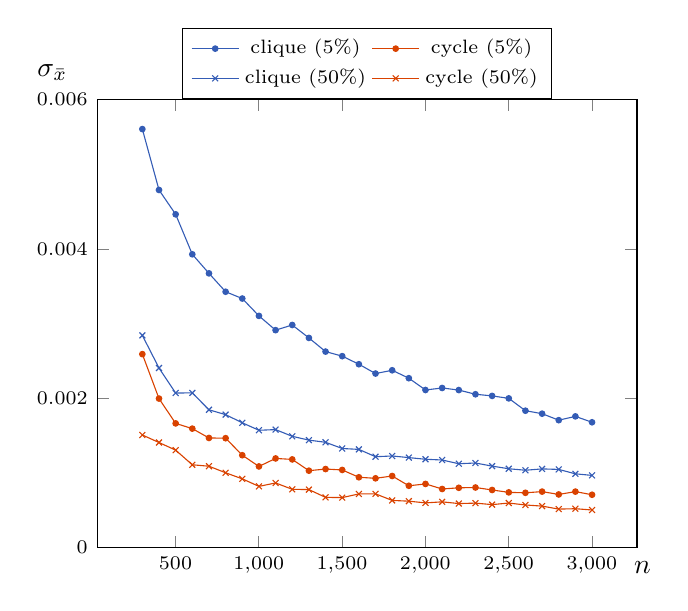
\begin{tikzpicture}
  \pgfplotsset{yticklabel style={/pgf/number format/fixed, /pgf/number format/precision=3}, scaled y ticks=false}
  \pgfplotsset{every axis legend/.append style={at={(0.5,1)},anchor=south}} %%% To put legend outside the box
\begin{axis}[legend columns=2, %%% Legends horizontally
        %axis equal image=true,unit vector ratio=9 1,width=1.1\columnwidth, %%% size of box
        ymin=0,
        ymax=0.006,
        every tick label/.append style={font=\scriptsize},legend style={font=\scriptsize}, %%% size of legends
        xlabel=$n$, ylabel=$\sigma_{\bar{x}}$, %%% axis labels
        every axis y label/.style={at={(ticklabel cs:1.02)},anchor=south west}, %%%% position of y-axis legend
        every axis x label/.style={at={(ticklabel cs:1.01)},anchor=south}, %%%% position of y-axis legend
        ]
    %\draw[help lines] (axis cs:0,1) -- (axis cs:3,1);
\addplot[color=\cliquecolor,mark=*,mark size=1pt] coordinates {
  (301, 0.005602)
  (401, 0.004787)
  (501, 0.004461)
  (601, 0.003926)
  (701, 0.003671)
  (801, 0.003425)
  (901, 0.003334)
  (1001, 0.003102)
  (1101, 0.002911)
  (1201, 0.002980)
  (1301, 0.002807)
  (1401, 0.002624)
  (1501, 0.002563)
  (1601, 0.002455)
  (1701, 0.002330)
  (1801, 0.002374)
  (1901, 0.002268)
  (2001, 0.002110)
  (2101, 0.002137)
  (2201, 0.002109)
  (2301, 0.002053)
  (2401, 0.002031)
  (2501, 0.001998)
  (2601, 0.001833)
  (2701, 0.001793)
  (2801, 0.001706)
  (2901, 0.001757)
  (3001, 0.001678)
};
\addplot[color=\cyclecolor,mark=*,mark size=1pt] coordinates {
  (301, 0.002590)
  (401, 0.001995)
  (501, 0.001663)
  (601, 0.001593)
  (701, 0.001468)
  (801, 0.001465)
  (901, 0.001237)
  (1001, 0.001087)
  (1101, 0.001194)
  (1201, 0.001181)
  (1301, 0.001030)
  (1401, 0.001052)
  (1501, 0.001040)
  (1601, 0.000942)
  (1701, 0.000928)
  (1801, 0.000959)
  (1901, 0.000828)
  (2001, 0.000853)
  (2101, 0.000785)
  (2201, 0.000801)
  (2301, 0.000805)
  (2401, 0.000772)
  (2501, 0.000740)
  (2601, 0.000734)
  (2701, 0.000750)
  (2801, 0.000712)
  (2901, 0.000750)
  (3001, 0.000708)
};
\addplot[color=\cliquecolor,mark=x,mark size=1.5pt] coordinates {
  (301, 0.002841)
  (401, 0.002404)
  (501, 0.002070)
  (601, 0.002071)
  (701, 0.001845)
  (801, 0.001780)
  (901, 0.001671)
  (1001, 0.001571)
  (1101, 0.001580)
  (1201, 0.001490)
  (1301, 0.001439)
  (1401, 0.001410)
  (1501, 0.001327)
  (1601, 0.001315)
  (1701, 0.001217)
  (1801, 0.001227)
  (1901, 0.001205)
  (2001, 0.001183)
  (2101, 0.001173)
  (2201, 0.001123)
  (2301, 0.001133)
  (2401, 0.001091)
  (2501, 0.001056)
  (2601, 0.001036)
  (2701, 0.001054)
  (2801, 0.001047)
  (2901, 0.000988)
  (3001, 0.000967)
};
\addplot[color=\cyclecolor,mark=x,mark size=1.5pt] coordinates {
  (301, 0.001508)
  (401, 0.001407)
  (501, 0.001305)
  (601, 0.001109)
  (701, 0.001090)
  (801, 0.001002)
  (901, 0.000921)
  (1001, 0.000820)
  (1101, 0.000866)
  (1201, 0.000781)
  (1301, 0.000777)
  (1401, 0.000673)
  (1501, 0.000670)
  (1601, 0.000719)
  (1701, 0.000720)
  (1801, 0.000632)
  (1901, 0.000622)
  (2001, 0.000599)
  (2101, 0.000613)
  (2201, 0.000590)
  (2301, 0.000596)
  (2401, 0.000576)
  (2501, 0.000597)
  (2601, 0.000571)
  (2701, 0.000556)
  (2801, 0.000516)
  (2901, 0.000521)
  (3001, 0.000504)
};
\legend{clique (5\%), cycle (5\%), clique (50\%), cycle (50\%)}
\end{axis}
\end{tikzpicture}
\end{document}
